\documentclass[11pt]{article}
%Required: You must have these
\usepackage{graphicx}
\usepackage{tabularx}
\usepackage{natbib}

\usepackage{array}
\usepackage{amsmath}
%\usepackage[backend=bibtex]{biblatex}
\setkeys{Gin}{width=0.8\textwidth}
%\setlength{\captionmargin}{30pt}
\setlength{\abovecaptionskip}{10pt}
\setlength{\belowcaptionskip}{10pt}
 \topmargin -1.5cm 
 \oddsidemargin -0.04cm 
 \evensidemargin -0.04cm 
 \textwidth 16.59cm
 \textheight 23.94cm 
 \parskip 7.2pt 
\renewcommand{\baselinestretch}{1.2} 	
\parindent 0pt


\bibliographystyle{..//refs/styles/besjournals.bst}
%\usepackage{xr-hyper}
\usepackage{hyperref}
\title{Experimental designs for testing the interactive effects of temperature and light in biology(ecology) and the problem of periodicity }
\begin{document}
\maketitle
\section{Introduction}
Temperature and light dictate numerous biological processes including....\textit{list here}\citep{}. These cues often interact in complex ways, and a major goal of biology is to quantify their both individual and interactive effects on biological activity \citep{}. This effort has only become more critical in recent decades as such measurements are essential for accurately predicting organisms' response to anthropogenic global change and informing biodiversity conservation planning and practices \citep{}.\\

It is difficult to evaluate the individual effects of temperature and light cues and their interactions in \textit{in situ} observational studies because temperature and light variables tend to co-vary in nature \citep{}. However, well designed experiments in controlled environments (e.g. growth chambers, greenhouses, mesocosm) can be used to manipulate temperature and light variables independently, allowing for robust comparisons of their individual and interactive contributions to biological processes. Indeed, this approach has provided many fruitful insights regarding temperature and light signaling over the last century \citep{} and has great potentially to continue to advance fundamental and applied biological inquiries in the decades to come \citep{}.\\

However, controlled environment experiments have their own challenges. Experimentalists must balance biological realism with statistical inference \citep{}, experimental effort with statistical power \citep{} and account for the effects of unmanipulated or unmeasured variables \citep{}. Below we highlight a particular challenge that can arise in experiments seeking to estimate the interactive effects of temperature and light on biological outcomes when the periodicity of both variables is included. Our example deals with the phenology (timing of recurring life cycle events, e.g. leaf budburst, flowering) in temperate woody plants and for a brief overview of how temperature and light interact to influence phenology see the Suppliment. However, the issues and solutions we present below are broadly applicable to studies of any other organisms and biological processes that utilize temperature and daylength signals \citep{}. \\

We begin by reviewing the minimum experimental elements required to robustly test interactions between two or more variables. We then detail the problem of inference that can arise manipulating the periodicity of both temperature and light in experiments and demonstrate the extent to which this is an issue with a mathematical and experimental example. Finally, we conclude by outlining several possible solutions for overcoming these issues. 

\section{Testing interactions in contolled environmental}
In order to have the statistical power to partition the individual and interactive effects of two or more variables in an experiment, one must:
\begin{enumerate}
\item Have at minimum of two treatment levels of at least two variables \citep{}.
\item Treatment levels must be full factorial (Fig. \ref{examp}a.). Full factorial designs are both balanced (Fig. \ref{examp}b.)  and orthogonal (Fig. \ref{examp}c.); which is to say that all possible treatment combinations are applied and each treatment is independent of all others \citep{}.
\end{enumerate}

These two critical elements may seem obvious but can be conspicuously absent from many published studies. In the case of woody plant phenology, using a recently published database (OSPREE: Observed spring phenolgoical responses in experimental enviornments \citep{}) we found that out of 136 controlled environment studies \citep{}, only 21 of them manipulated both light and temperature cues in the same experiment and only 17 of those did so with a design that was both balanced and orthogonal (see Supplement for details). This notable dearth of robust tests of light and temperature interactions may stem from the common limitations of time, space, and resources that experimentalists often face \citep{}, but it may equally relate to a fundamental issues that arises from the fact that these variables themselves are comprised of multiple axes of variably.

\section{Axes of environmental variation in experiments and their implications}
For most environmental variables, including light and temperature, there are two major axes of variation that can be manipulated in an experiment.  
\begin{enumerate}
\item \underline{Intensity:} The amount or quality of a variable. Here we define temperature intensity as the amount of heat present in the system (measured in degrees).  In the phenology literature this measurement is generally referred to as forcing. We define light intensity as the luminosity or irradiance present in the system (measured in lumens or watts). 
\item \underline{Periodicity:} The interval at which the intensity of the variable is applied. Hereafter, we refer to the periodicity of light as photoperiod (often used synonomously with ``daylength") and the periodicity of temperature as thermoperiod. 
\end{enumerate}
\textit{(sentence here backing down from above statment and aknowldge there are other axes especiall with light)}
For phenology, it is generally accepted that photoperiodicity is the primary light cue to which plants respond (\citep{} though see \citep{} regarding light intensity and phenology). For temperature, conventionally both intensity and periodicity drive phenological activity \citep{} and several metrics, (e.g. growing degree hours, thermal sums, growing degree days)  that combine these two axes have been developed \citep{}. This assumption is well supported; under natural conditions diurnal temperature fluctuations in temperate regions can be quite large in the spring, and several studies have found that diurnal temperature variation strongly influences plant phenology \citep{}. In fact, several studies suggest that the even if thermoperiodicity is not an explicit treatment variable (i.e. manipulated systematically), incorporating it in experiments is essential for translating experimental results into real world predictions \citep{}.

It follows that a common approach in phenology experiments that seems to balance prior knowledge, biological realism and experimental inferences is to vary photoperiodicity, and thermal intensity and periodicity \citep{}. For example, a basic experiment might include a long (12 hours) and short (8 hours) photoperiod treatment and a high (30/20$\degree$ C day/night) and low (20/10 $\degree C$ day/night) temperature treatment. Note that in this case, the thermoperiodicity is not an explicit treatment (both high and low temperature treatments employ a diurnal fluctuation of 10 $\degree$ C), and is simply incorporated in the design to enhance biological realism. At first glance, this design appears to meet the criteria of a full factorial design, multiple treatment levels that are balanced and orthogonal, with mean high/low temperature treatments (25 and 15 $\degree$ C respectively) and long/short photoperiod treatments applied in all possible combinations.

Yet the orthogonality of this design is based on the assumption to a 12 hour thermoperiod. If, rather the thermoperiod is coupled with the photoperiod, orthogonality is violated, in that the daily mean temperature of the long/high treatment will be higher than that of the short/high treatment, and the long/low treatment slightly warmer than the short low (Fig \ref{ortho}.a). This is because the warmer day time temperatures are applied for different duration across the high temperature treatments. Ultimately, this non-orthogonality introduces covariation among the photoperiod and temperature treatments, making it statistically impossible to differentiate their independent and interactive effects.\\

Of the studies in the OSPREE database that manipulated both photoperiod and temperature interactively, we found that around 30\% of them may have this issue, suggesting that the true interactive effects of these cues on spring phenology is still quite poorly characterized. This may be in part why the relatively contribution of temperature and photoperiod cues to spring phenology remains a contentious debate in the phenology literature \citep{}.

\section*{Quantifying the uncertainty}
To estimate the potential impact of this experimental artifact on estimations of cue effects, we used the simple geometry of a plane to calculate the approximate maximum amount of the forcing (temperature) and photoperiod effect estimates that could potentially be mis-attributed due to the latent non-orthogonality of in a coupled therm0-photoperiod design. We based our calculations on estimates from the a study by \citet{} in which the forcing and photoperiod effects on spring phenology were estimated to be approximately -9.5 and -4.5  $\Delta$ day of leaf out / $\Delta$ cue level. Our calcuations suggest that as much about 3.0 units of of these effects could be mis-attributed from a coupled photo-theromoperiod experiment (for the full calculations see the Supplement.) Because forcing is expected to be the more dominant cue \citep{}, we would expect the covariation of these variables may result in an over-estimation of the photoperiod effect and a weaker interaction estimate. \\

%It is important to stress that this math is not meant to serve as rigid model correction. It is certainly possible that original model estimate approach the ``true" values,  but, due to the covariation of thermo- and photoperiod there is no way of knowing for certain. (\textit{Probably should think about how to phase all this without making it seem like the Flynn paper is bad or wrong}).\\

Our estimate of ``how much of each cue estimate could be mis-attributed to the covariation of thermo- and photoperiod" can be rephrased as a maximum prediction of the expected difference in effect size estimates from a coupled photo- and thermo-period experiment and an uncouple one in which diurnal photoperiod and thermoperiod are varied independently. While we are aware of no experiments that explicitly compare these different designs, another later study by \citet{Buonaiuto2020} utilized many overlapping treatment levels and species from the same sampling site and several treatment levels with the \citet{Flynn2018} study, but authors decoupled photo- and thermo-period,  allowing for a reasonable comparison.\\ 

We subset each dataset (publicly available at  HF and KNB ) to include only the  species shared among the two studies, and re-analyzed the data using Bayesian hierarchical models to compare difference in the photoperiod and forcing  estimates (see Supplement for Methods).  We found that the estimated differences in the mean response to photoperiod, forcing and their interactions amoung study designs were on the same order our mathmatical predictions, and that the un-coupled design estimated a weaker (less negative) photoperiod effect, and stronger forcing and interaction effects than the coupled experimental design (\ref{fig:compy}). \\

It is worth saying that there may be other factors driving the differences between these experiments.  For example, both were conducted in different years, sampled different individual from the population, and used different methods for applying an addition temperature pre-treatment ,chilling (see Supplement). However, becasue this comparison is well matched to our mathematical predictions and prior knowledge about how temperature and photoperiod are expected to interacting in phenology, we argue that the influence of periodicity covariation on statistical inference is apparent enough to take seriously .\\

\section{Paths Forward}
In the sections above we have systematically demonstrated that experiments which co-vary thermoperiod and photoperiod cannot robustly differentiate the individual effect of temperature and photoperiod on a spring phenology (or any other biological process) or quantify their interactive influence. Given the paucity of interactive studies in the literature, it is clear that more well designed studies will be needed to better characterize the effects of these cues. Below we offer several generalized experiment designs that improve statistical orthogonality of controlled environment experiments which could be further developed and adjusted to fit the needs of experimentalists across many sub-fields of biology.
\begin{enumerate}
\item \textbf{Manipulate photoperiod and temperature intesity with no thermoperiodicity}. This approach allows for the maintenance of statistical orthogonality across treatment combinations (\ref{fig:ortho}b.). The main drawback is that this design sacrifices the biological realism of diurnal temperature variation, which may make it more difficult to translate estimates from experiments to real world applications.

\item \textbf{Compensitory diurnal temperature fluctions}. There are almost unlimited pairs of integers that can reduce to the same mean (e.g. $(24+26)/2 = (30+20)/2 = 25$) and the non-orthogonality of the mean daily temperature that arises in a coupled photo-thermoperiod design could be corrected for by proportionately increasing the diurnal temperature fluctuation of the short photoperiod treatment relative to the long treatments (\ref{fig:ortho}c.). However, if the differences between day and night temperature has a meaningful biological effect \citep{}, this introduces another confounding, non-orthogonal factor for interpreting temperature and photoperiod effects. For example, the influence of day time warming of phenology can be as much as three times stronger than proportionate night time warming \citep{}.

\item \textbf{Uncouple thermoperiod and photoperiod.} By varying thermoperiod and photoperiod independently (\ref{fig:ortho}d.), statistical orthogonality can be maintained across treatment. However, this approach may also introduce new artifacts that occur from the biological rather than statistical interactions between light and temperature. For example, there is evidence that increasing temperatures in the first two hours of daylight can be almost as effective for stimulating shoot elongation as similar temperature increases for the whole photoperiod \citep{Erwin1998}. With this design, treatments must inherently differ in the amount of time the warmer daytime temperature extends into the dark nighttime light regime, introducing a new axes of non-orthogonality.
\end{enumerate}

In correcting one problem, each on of these designs introduces another, which may in fact be an intrinsic property of any experimental manipulation. This fact should caution experimentalists to continue to think carefully about our designs and perhaps most importantly, remind us to be humble in our inference, and think critically about what is, and isn't accounted for in our work. 


\begin{figure}[h!]
    \centering
 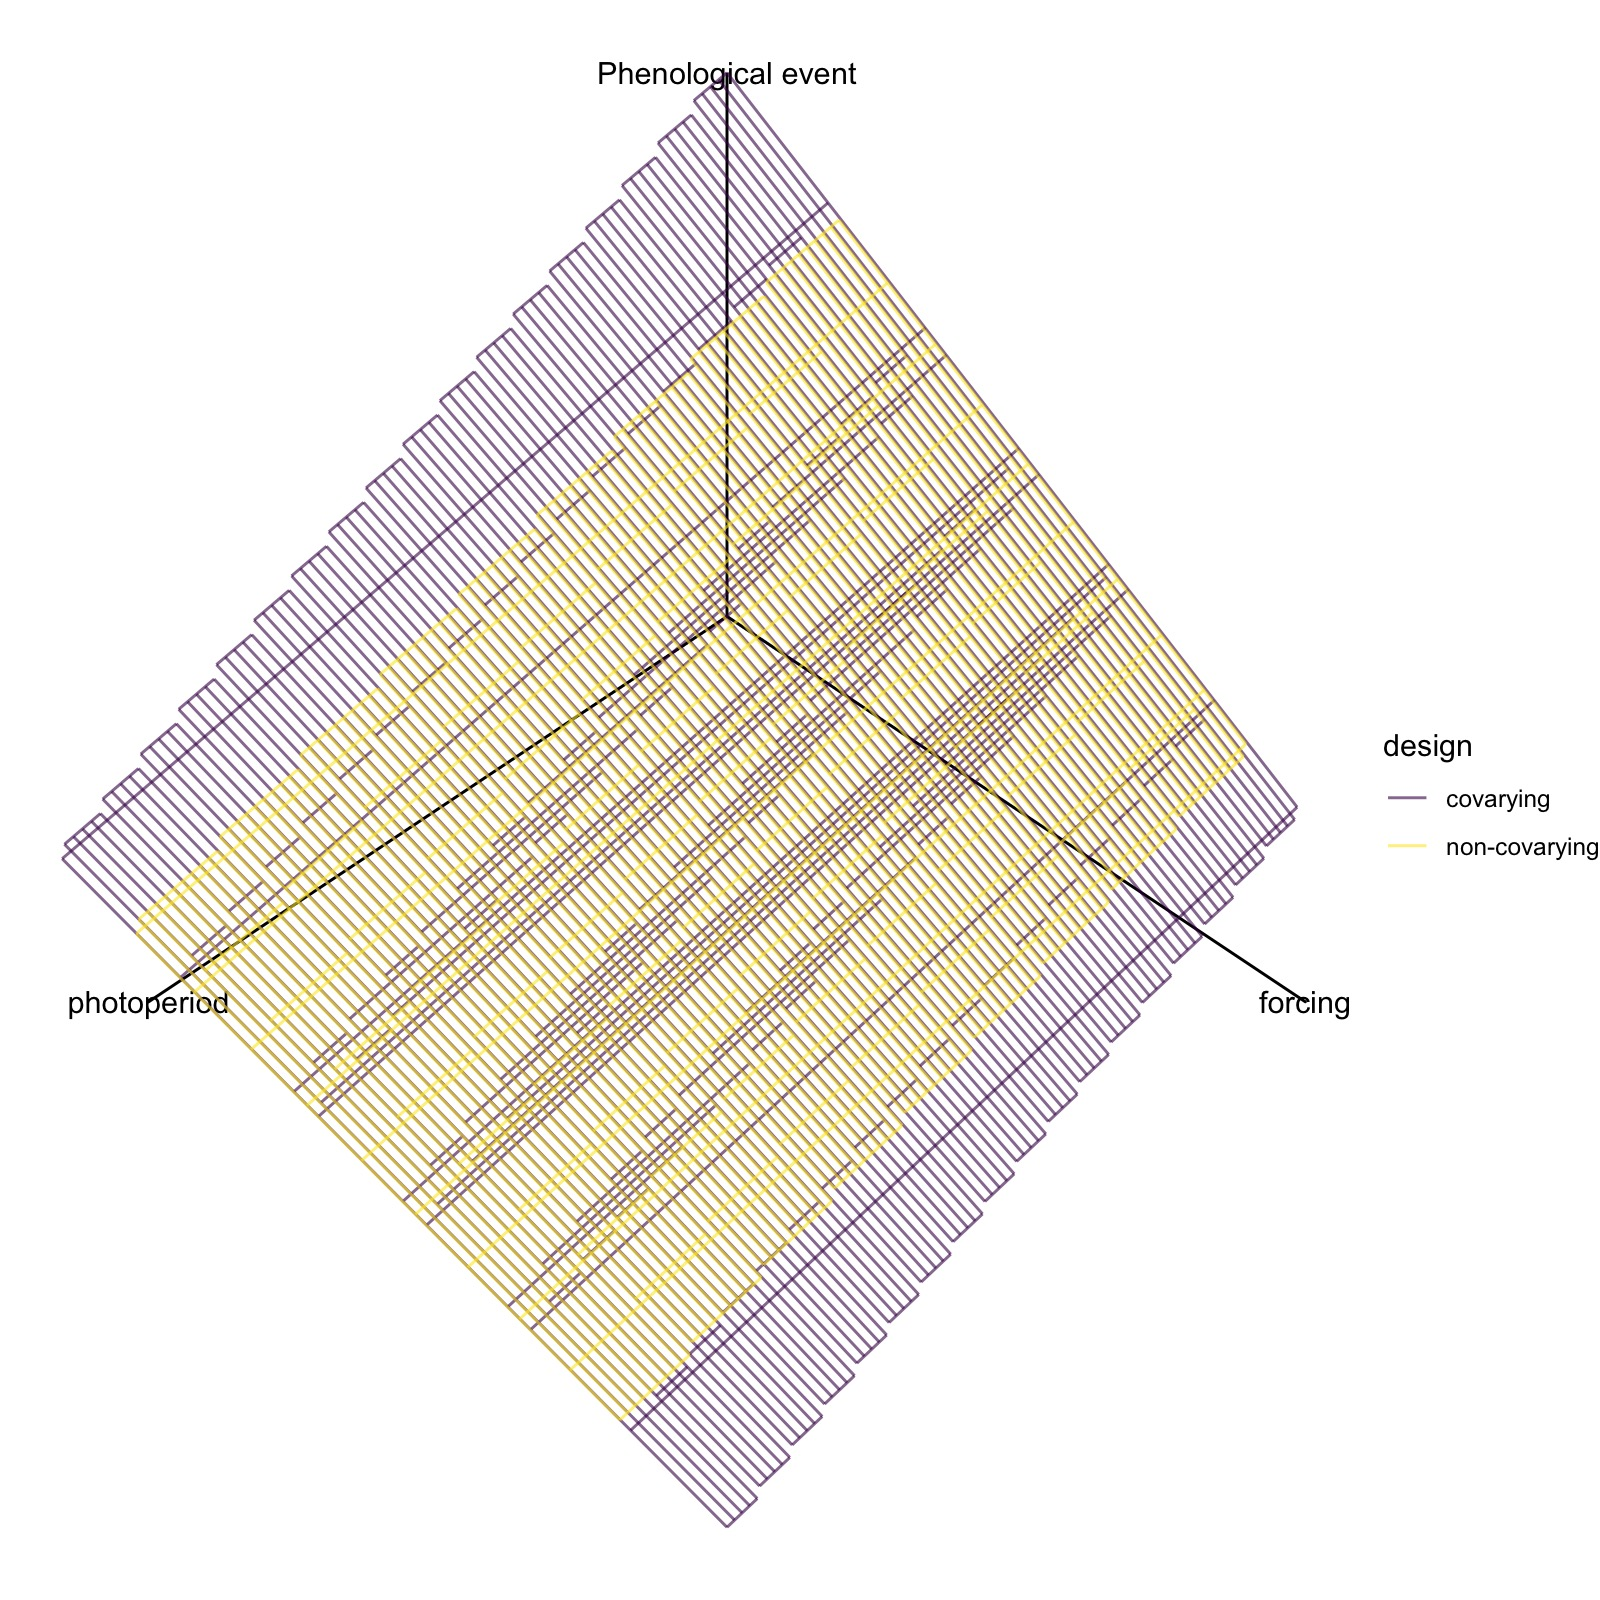
\includegraphics[width=.8\textwidth]{..//Plots/periodicity_figures/orthog.jpeg}
    \caption{Idealized experimental designs demonstrate three approaches for varying temperature and light treatment level in controlled environment experiments. Design \textbf{a)} is fully factorial in that treatments levels are balanced and orthogonal. This design is appropriate for testing interactions between two or more variables. In \textbf{b)} the design is balanced both not orthogonal. Non-orthogonality in experiments often arises in experiments when there is covariation among the test variables is unaccounted for. In \textbf{c)}, the experimental design is orthogonal but unbalanced. Lack of balance in experiments often arises due to time, space or resource limitations. }
    \label{fig:examp}
\end{figure}

\begin{figure}[h!]
    \centering
 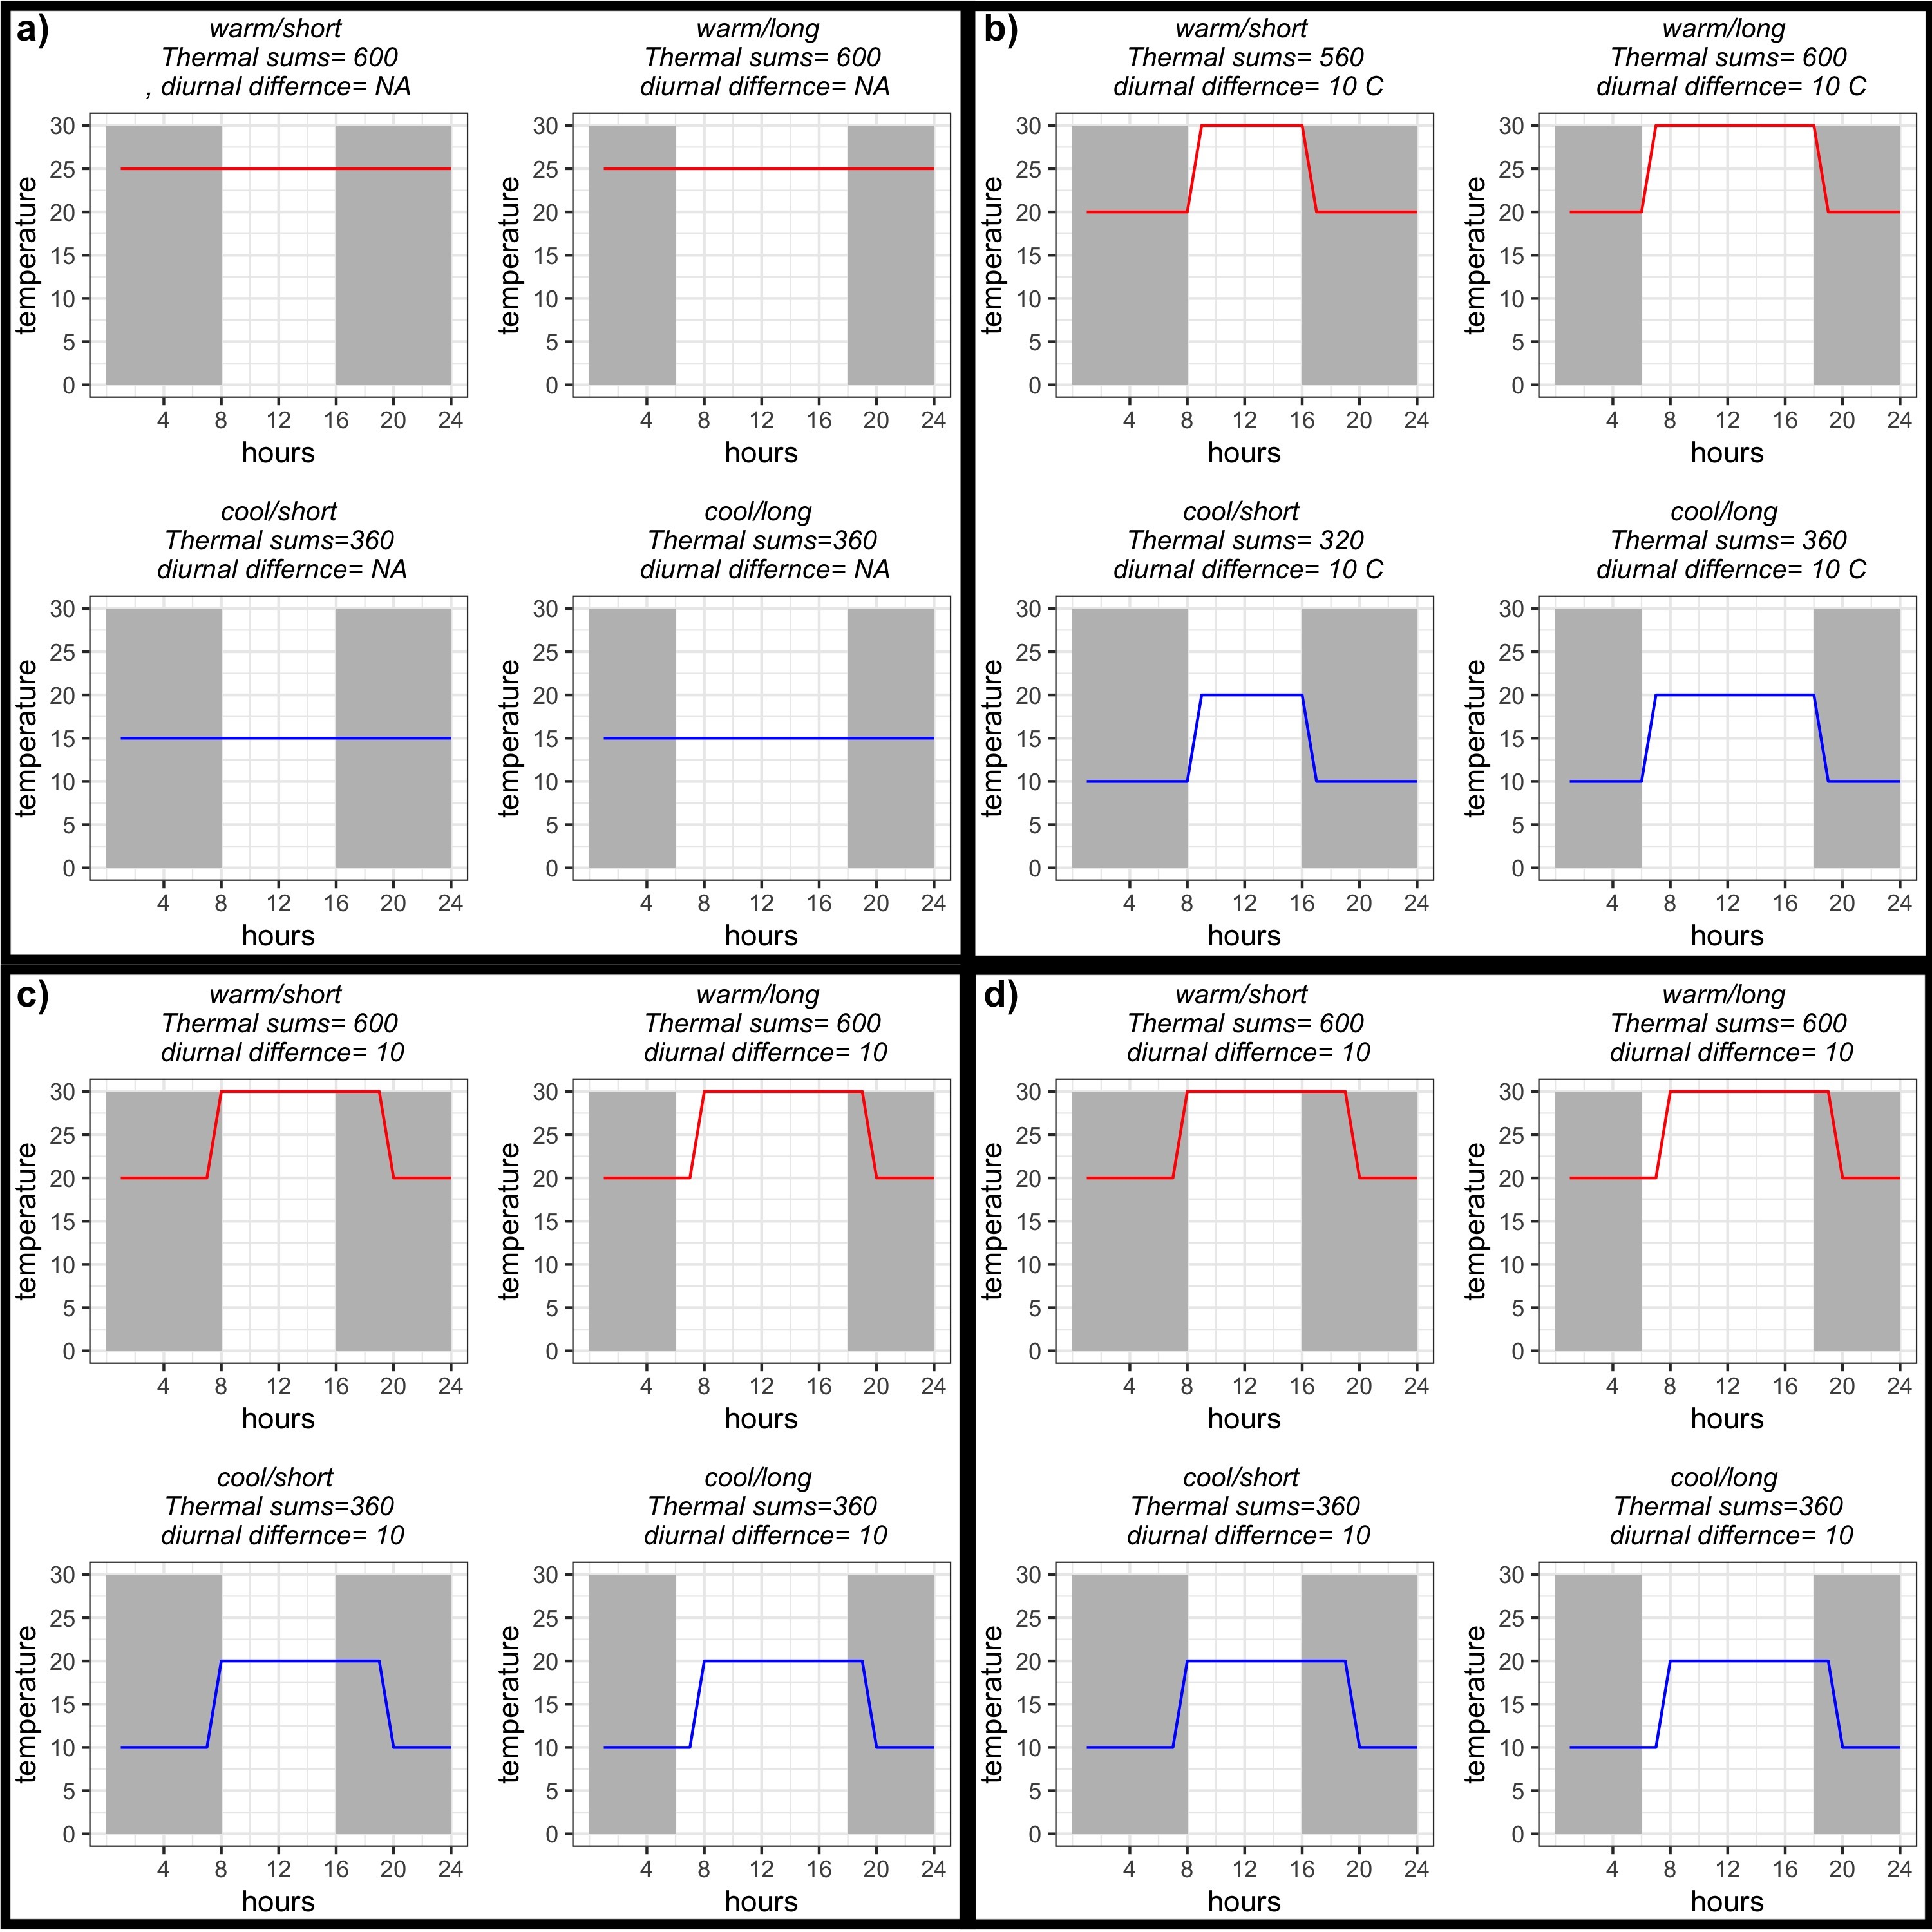
\includegraphics[width=\textwidth]{..//Plots/periodicity_figures/designs.jpeg}
    \caption{Conceptualized experimental designs to test temperature and daylength interactions on a biological response. In \textbf{a)} the design incorporates a standardize diurnal temperature fluctuation across all treatment. Because this thermoperiod is coupled with the photoperiod, while the same day and night temperatures are applied for the high and low temperature treatments respectively, the mean daily temperatures differ across each photoperiod treatment generating non-orthogonality. Designs \textbf{b)},\textbf{c)} and \textbf{d)} are all designs that can  correct this non-orthogonality. Design \textbf{b)}  manipulated temperature intensity only (no thermoperiodicity).% sacrificing some biological realism if the biological response in question requires diurnal temperature fluctuations. 
    In  \textbf{c)} photo- and thermo- periods are still are coupled but the orthogonality of mean daily temperature is maintained by proportionately varying the diurnal temperature fluctuations across treatments. %However, if temperature and light intensity interact biologically, this approach introduce unbalance and non-orthogonality introducing a new latent difference among the treatments in the form of diurnal temperature range.
    In design \textbf{d)} standard diurnal temperature fluctuations are maintained but, thermoperiod and photoperiod are decoupled and varied independently, maintaining orthogonality daily mean temperatures.}% but may introduce inferential bias as the periodicity of temperature relative to temperature will be non-orthogonal among treatment combination.} 
    \label{fig:ortho}
\end{figure}
 
\begin{figure}[h!]
    \centering
 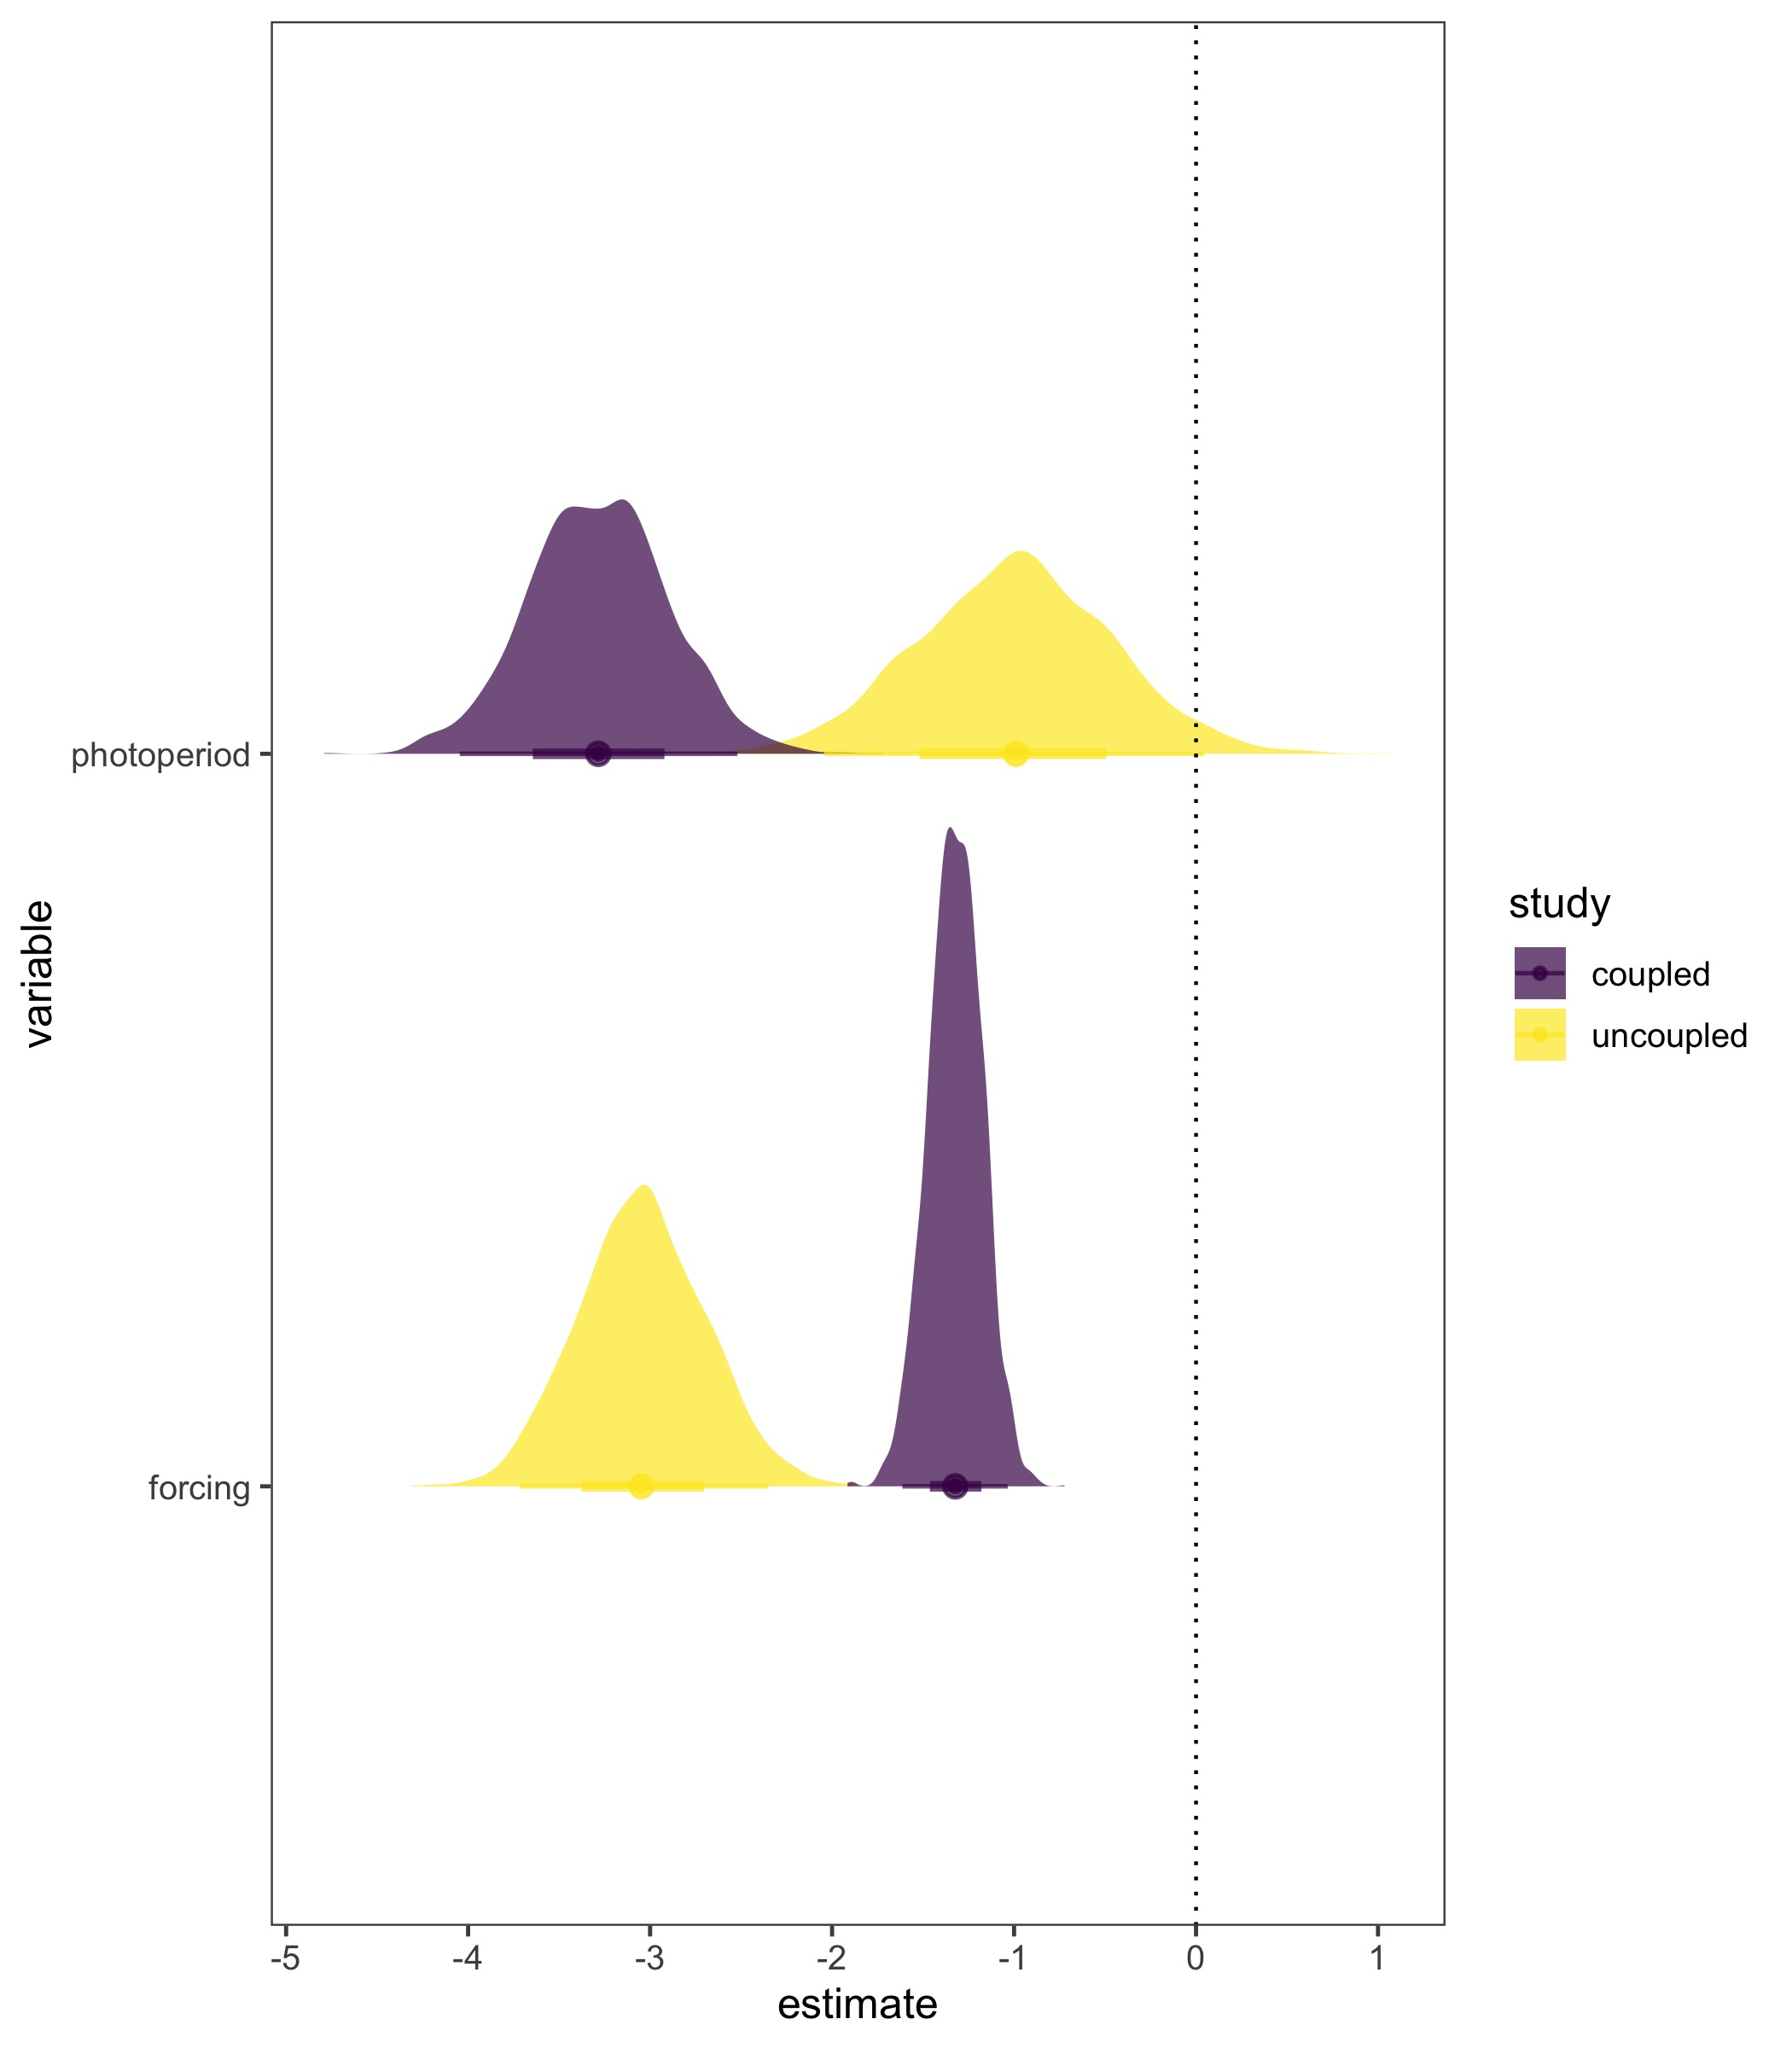
\includegraphics[width=\textwidth]{..//Plots/periodicity_figures/modelcomps.jpeg}
    \caption{Need a caption but basically, estimates differs in expected ways} 
    \label{fig:compy}
\end{figure}
 

\end{document}




\begin{enumerate}
\item Temperature and light control and signal many biological processes.
\item They often interact, substitute or compensate for each other.
\item A major goal of biology is to quantify their effects and interactions
\item This has become extra important for predicting organism's response to global change
\item This task cannot be done well through observational studies as light and temperature regimes usually co-vary
\item Experiments in controlled environments (growth chambers, greenhouses etc) can do this, using experimental treatment to partition the effects of this variables and their interactions.
\item Indeed much progress has been made with this approach
\item But experiments must balance many competing factors in their designs, biological realism with statistical inference, the effect of unmeasured climate variable, blocking effects etc.
\item In the sections below we highlight a particular problem that can arise when designing experiments to partition the effects of temperature and daylength and understand their interaction. Our example uses woody plant phenology as an example, but the approach we detail here is relevant for other organisms and biological process too.  
\end{enumerate}

\section{Phenological response to Temperature and Light}
Here a very brief (one paragraph) overview of how light and temperature influence spring phenology. Keep it basic (Warming accelerate phenology, photoperiod might be a threshold), aknoledge chilling is important too, but our example won't really focus on it. Leave some open questions about their interactive nature.

\section{Testing Interactions}
\begin{enumerate}
\item To test interactions and partition effects amoung two variables that covary in nature one must:
\item Have at least 2 treatment levels of each variable of interest
\item Apply them orthoganigally, factorially (\ref{fig:examp}, blue box) and define these terms.
\item This may seem obvious but is rarely done. In the case of phenology, a recent analysis of controlled enviroonment study found that only X of Y studies manipulated both light and temperature cues in the same experience and only Z of X did so orthoginally.
\end{enumerate}
\section{Axes of environmental variation annd their there problem}
\begin{enumerate}
\item A further complication arises when decided how to apply each treatment.
\item For any environmental variable there are two axes of variation that can be manipulated in an experiment.  
\item Intensity: Temperature, luminocity. 
\item Period: Thermoperid, Photoperiod.
\item There are measures that incorperate both period intensity (ie growing degree hours).
\item For light cues, photoperiod is the primary phenolgoical cure
\item For temperature, period and intesity matter. For example, temperture in nature varies diurnally and dirunal temperature fluctions may contribute to the phenology signal, or at the very least, lack of them might make phenology wonky. 
\item Therefore a common approach in experiments that seems to balance prior knowlege, biological realism and experimental inferences is to vary photo period, and temperature intensity and period. 
\item Clarify with an example. 12 and 8 hours of daylength. 30/20 and  20/10 temperature (or whatever I said in the figure).
\item If not carefully handled this approach can introduce a nonorthogicanity into the experiment, biasing inference.
\item If the thermo-periodicity and photoperiodcity are coupled (ie the night time temperatures begin when the lights go off, and the day time temperatures begin when they turn back on) The impact is that that the high temperautre high/long photoperod treatment more cumulative heat than the high temperature/short photoperiod treatment throughout the experiment as can be seem when the temperature treatment are converted to thermal sums (\ref{fig:examp},(\ref{fig:ortho}b)). To state this more simply, though the applied temperatures are the same sicne their are applied for different durations, the mean daily temperature differ among the temperature treatments.
\item This non-orthoginality makes it stasticially impossible to differentiate the effect of the photoperiod and temperature treatments.
\end{enumerate}
\section{Quantifying uncertainty}
\begin{enumerate}
\item To estimate the extent to which this non-orthangonical could bias results we intergated the results from a large scale experiment that included a coupled thermo-photoperid design. We used plane geometry to estimate how much of the estimated forcing effect (the assumed dominant cue) may actually be attributed to change in photoperiod. The calcualtions can be found in the suppliment.
\item While the original model estimates of the forcing and photoperiod effects (phenological sensitivy; $\Delta$ phenological event day/ $\Delta$ cue level) were estimate 9.5 and 4.5 advance we estimate that as much about 3.0 (units?) of the forcing effect could be attributed to the photoperiod effect.
\item It is important to stress that this is not a model correction. The original model could acutally before correct or it could in fact have understimated the true forcing effect and infalted the photoperiod effect. We simply cannot say this. (\textit{Probably should think about how to phase all this without making it seem like the Flynn paper is wrong}).
\item Our estimate of ``how much of the reported photo-period response could in actuality be driven by the latent differences in thermo-period" can be rephrased as a prediction of the expected difference in estimated photoperiod sensitivity between a coupled and decoupled photo- and thermo-period experiment.
\item While we are aware of no experiments that explicitly test these different designs, a phenological study by \citet{Buonaiuto2020} applied serveral treatments levels that overlap with those in the \citet{Flynn2018} study to twig cuttings from the same source population. However in the second study the authors decoupled photo- and thermo-period. After subseting each dataset to  include nly species and treatment levels common amoung them, we re-analyzed the data (see supplimental method) and found that difference in the average response to photoperiod amoung study designs  was on the same order our mathmatical prediction see figure, though the photoperiod effect was in fact weaker in the uncoupled dataset (\ref{tab:compy}).\\
\item  With such significant uncertainty in partitioning the effect of forcing and photoperod even in experiment, this might contribute to the debate about the importance of photoperiod.
\item Below we outline several solutions to this experimental design, that should inprove the inference from growth chamber studies
\end{enumerate}

\section{Solutions}
\begin{enumerate}
\item Manipulate temperature intesity only and photoperiod. You estimate interactions because you have multiple levels of temperature and orthogiality. Lose some biological realism (\ref{fig:ortho}a).


\item Uncouple thermoperiod and photoperiod. As done in \citet{Buonaiuto2020}. While this is probably better than coupled approach as it account for statistical interaction, it may introduce new artifact that occur from biological interactions. For example evidence from horticulture studies have demonstrated that cell growth is most sensitive to temperature fluctuation at the beginning of the photoperiod\citep{Erwin1998}. \citet{Erwin1998} found that increasing temperatures in the first two hours of the photoperiod was almost as effective for stimulating shoot elongation as similar temperature increases for the whole photoperiod (\ref{fig:ortho}c).

\item Set temperature treatments using metrics that account for period and intestist. Growing degree hours.maintain mean temperature and set photoperiod legnths and thus thermal orthoginality in expiriment by proportionately varying diurnal fluctionation accross treatment level. However, if the differenes between day and night temperature has a meanful biological effect as has been shown, this introduces another confonding, non-orthoginal factor (\ref{fig:ortho}d).

\item While this improvements should improve our ability to assess light and temperature interactions in biology, their challenges should aslo remind us to be humble with inference and think critically about what is, and isn't accounted for.
\end{enumerate}


